121.\begin{figure}[ht!]
\center{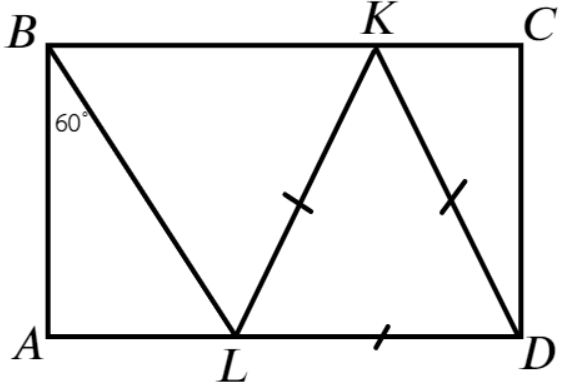
\includegraphics[scale=0.35]{g8-119.png}}
\end{figure}\\
Так как $KD=DL=KL,$ треугольник $KDL$ является правильным и все его углы равны по $60^\circ,$ тогда $\angle KDC=90^\circ-60^\circ=30^\circ$ и $CD=KD\cos(30^\circ)=8\cdot\cfrac{\sqrt{3}}{2}=4\sqrt{3}=AB,\ AL=AB\ tg(60^\circ)=4\sqrt{3}\cdot\sqrt{3}=12.$ Таким образом, $S_{ABCD}=AB\cdot AD=4\sqrt{3}\cdot(12+8)=80\sqrt{3}.$\\
